%!TEX root = twig-gpu.tex

\section{Code generation}
\label{sec:code-gen}

To generate code, Twig uses an abstract, language-independent system with a small number of basic operations. The relative simplicity of the model is motivated by Twig's semantics, described in Sec.~\ref{sec:semantics}. It is helpful in clarifying the precise operations which Twig supports, without getting bogged down in the (potentially quite complicated) details of outputting code for a particular language.

Twig generates code in units called \emph{blocks}. A block of code represents anything that performs some operation on a set of inputs in order to produce a set of outputs. Blocks have zero or more inputs and/or outputs. Blocks can be combined in two different ways: \emph{sequentially}, or \emph{in parallel}. These operations are described below.

Our current implementation of this model generates C code, although the model is general enough to generate other languages as well. Figures \ref{fig:codegen}(a) and \ref{fig:codegen}(b) each depict a different basic block that generates C.

\subsection{Block Composition}

As mentioned above, Twig provides two fundamental operations on blocks. The first is\emph{sequential} composition, which we represent formally as addition ($+$) on blocks. Sequencing connects two blocks of code by ``wiring'' the outputs of the first block into the inputs of the second (see Fig.~\ref{fig:codegen}(c)). In C, this is done by creating uniquely-named temporary variables which are substituted into the original blocks.

The second operation is \emph{parallel} composition, where two blocks are combined so as to execute independently of one another, but to appear as one single block (see Fig.~\ref{fig:codegen}(d)). We represent this operation as multiplication ($\times$).

\begin{figure}[ht]
\centering
\begin{tabular}{cccc}
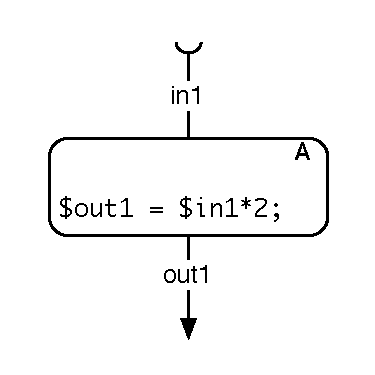
\includegraphics[width=1.1in]{images/codegen-a}& 
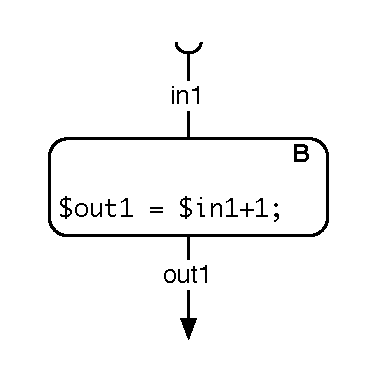
\includegraphics[width=1.1in]{images/codegen-b}& 
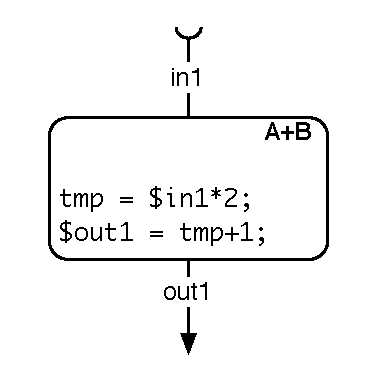
\includegraphics[width=1.1in]{images/codegen-seq}& 
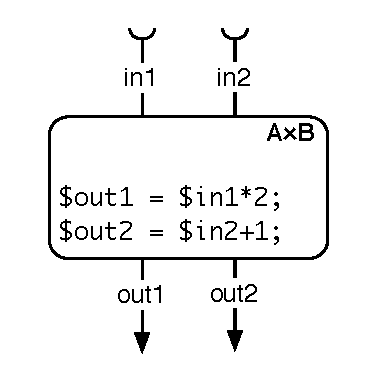
\includegraphics[width=1.1in]{images/codegen-par}\\
(a)&(b)&(c)&(d)\\
\end{tabular}
\caption{Code generation using blocks. $A$ (a) and $B$ (b) are basic blocks. $A+B$ (c) is the sequential composition of $A$ and $B$. $A \times B$ (d) is the parallel composition of $A$ and $B$.}
\label{fig:codegen}
\end{figure}


\subsection{Identity Blocks}

Twig's formal semantics require the definition of a set of special \emph{identity} blocks. An identity block $I_n$ has $n$ inputs and $n$ outputs ($n > 0$). Its function is, as its name implies, to simply pass each of its inputs through, unchanged, to the corresponding output. In Twig's semantics we use $I_n$ as a kind of ``no-op.'' We also use $I$ in place of $I_n$ when the value of $n$ is implied from the context.

Identity blocks are subject to a few rules, which we describe here informally and only briefly. First, $I_n$ are left- and right-identity elements under sequential composition, i.e., $I + x = x + I = x$ for all blocks $x$. Second, we can define parallel composition of identity blocks is defined by summing their size, i.e., $I_n \times I_m = I_{n + m}$.
